\section{Konkrete Datenmodelle}
\label{sec:concrete_model}

Die Datenmodelle welche die Informationen beinhalten aus denen der Generator ausführbaren Quellcode erzeugt, werden im folgenden Abschnitt erläutert. Dabei werden auch drei Entwurfsmuster vorgestellt welche in den Modellen Anwendung fanden, das Factory-Pattern \cref{sec:language_factory}, das Visitor-Pattern \cref{sec:language_visitor} und das Kompositum-Muster \cref{sec:language_model}.

\subsection{REST-Modell}
\label{sec:rest_model}

Zuerst muss die abstrakte Beschreibung der Spreadshirt-API von der XML-Form, bestehend aus einem \emph{WADL} (\cref{sec:wadl}) und einem oder mehreren Schemabeschreibungen (siehe \cref{sec:document_description_formats}), in ein für den Generator verarbeitbares Format überführt werden.

Die durch die WADL-Datei beschriebene Baumstruktur muss in ein Datenmodell bestehend aus Klassen und Objekten transformiert werden.
Um effektiv mit der XML Darstellung arbeiten zu können wird diese zuerst mit einem Parser (siehe \cref{sec:xml_parser}) in ein \emph{Document Object Model} (kurz DOM) überführt welches im Arbeitsspeicher gehalten wird und damit einen schnellen Zugriff für nachfolgende Operationen darauf erlaubt. In einem nächsten Schritt wird das DOM, welches noch viele XML spezifische Informationen enthält, auf die wesentlichen API beschreibenden Merkmale reduziert. Im Gegensatz zu der in \cref{fig:wadlstructure} veranschaulichten Webanwendungsbeschreibung werden Referenzen durch deren Definition im Modell ersetzt. Die Klassenamen des Datenmodells orientieren sich an den WADL Elementnamen.

\begin{figure}[tb]
    \centering
    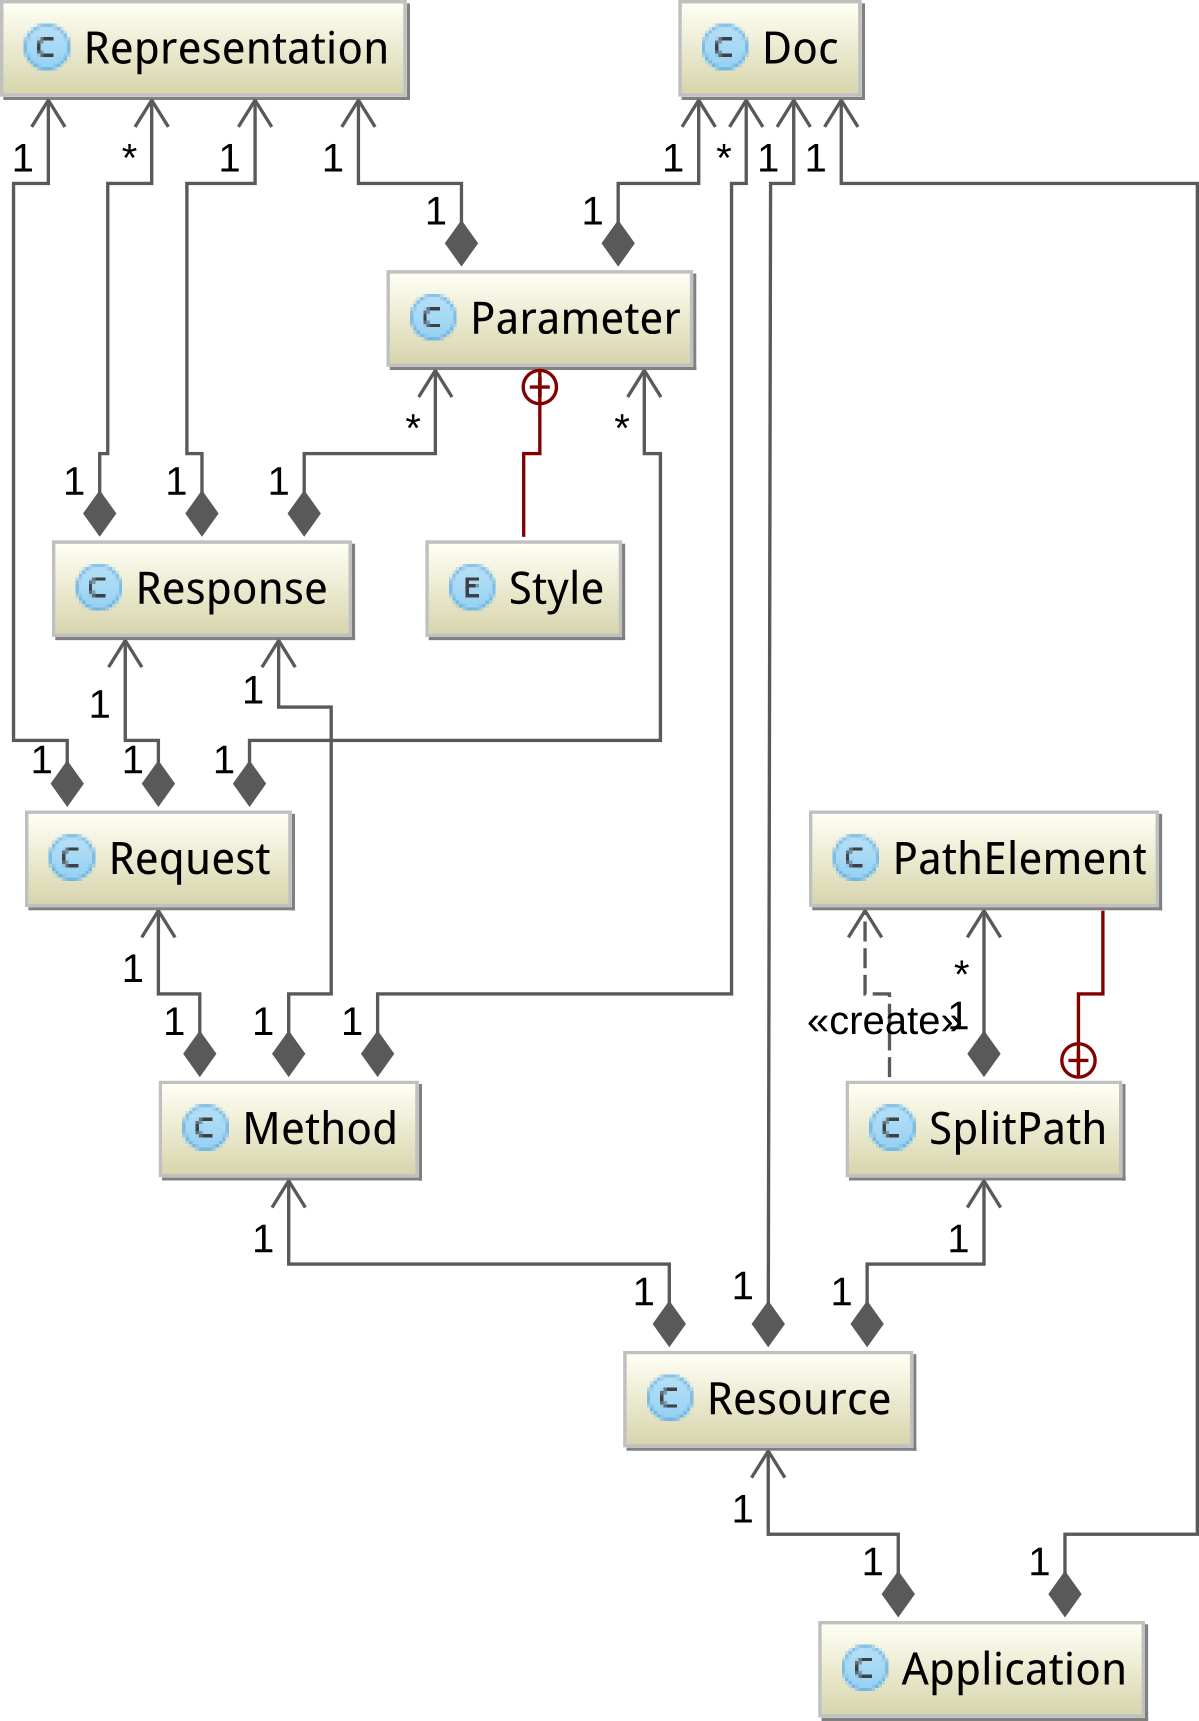
\includegraphics[width=0.5\textwidth]{resources/restmodel}
    \caption{UML Klassendiagramm des REST-Modells}
    \label{fig:restmodel}
\end{figure}

Wurzelelement des Modells (siehe \cref{fig:restmodel}) ist die Klasse \textbf{Application}, sie enthält \emph{Ressource}-Objekte und den Basisbezeichner der API bspw. \texttt{\small http://api.spreadshirt.net/api/v1/}. 

Eine \textbf{Ressource}-Klasse enthält eine Menge von \emph{Method}-Objekten, sowie einen Ressourcenbezeichner, dieser ist relativ zum Basisbezeichner des Wurzelelements. Die Ressourcenbezeichner können \emph{Template-Parameter} enthalten, diese werden bei einer Anfrage durch einen konkreten Wert ersetzt. Beispielweise enthält der Bezeichner für die Ressource eines bestimmten Users den Template-Parameter \{userid\}, vollständiger Ressourcenbezeichner \texttt{users/\{userid\}}. Ressourcenbezeichner werden durch die Klasse \textbf{SplitPath} repräsentiert. 

Jede \textbf{Method}-Klasse enthält ein \emph{Request} und ein \emph{Response} Objekt. Sie enthalten die nötigen Informationen für den Aufruf der Methode, bzw. über den Aufbau der Antwortnachricht.

Eine \textbf{Request}-Klasse enthält eine Liste von Query-Parametern sowie ein \emph{Representation} und \emph{Response} Objekt.

\textbf{Parameter} enthält Angaben zum \emph{Style}, Typ, Vorgabewert und ob dessen Angabe \enquote{required}, also notwendig ist. Die Angabe des Typs ist eine Referenz auf einen Typ aus einer XML-Schemabeschreibung. Der \emph{Style} gibt an wie der Parameter übermittelt wird, als Teil der Query \texttt{\ldots{}?mediaType=xml}, \emph{Key-Value Pair} des HTTP-Header oder als \emph{Template-Parameter} des Ressourcenbezeichners. 

Die Klasse \textbf{Response} enthält eine Liste mit \emph{Representation}-Objekten und Parameter-Objekten. Die Objekte vom Typ Representation enthalten die Beschreibung der Daten die bei einer erfolgreichen Anfrage an die Ressource zurückgesendet werden, sowie die der Fehlermeldung welche der Client anderenfalls erhält. Zwischen einer Fehlermeldung und einer erfolgreichen Anfrage kann anhand des Werts des HTTP-Statuscodes unterschieden werden. Erfolgreiche Anfragen liefern in der Antwort smeist einen Statuscode 200 \textbf{OK} oder 201 \textbf{Created} zurück, abhängig von der Anfragemethode. Die Response Parameter geben Einträge im HTTP-Header an, welche für den Client nützliche Informationen enthalten. Legt der Client z.B. via POST auf der Ressource \texttt{sessions} eine neue API-Session an, so enthält das Feld \texttt{Location} des HTTP-Headers der Serverantwort eine URL auf die Ressource der angelegten Session.

Die \textbf{Representation}-Klasse dient zur Beschreibung der Daten welche entweder zur API gesendet oder von dieser empfangen werden, sie besteht aus einer Angabe des \emph{media-type}, des HTTP-Statuscodes und eine Referenz auf die Definition des Datentyps. Das \emph{Representation}-Objekt des Request einer PUT- oder POST-Methode charakterisiert zum Beispiel den Aufbau der Daten welche der Ressource übermittelt werden, üblicherweise im HTTP-Body. Die Charakterisierung erfolgt dabei in Form einer Referenz auf einen Typ aus einer Schemabeschreibung sowie der Angabe des \emph{media-type}. Beispielsweise enthält das \emph{Representation}-Objekt der PUT-Methode auf Ressource \texttt{users/\{userId\}/designs/\{designId\}} den media-type \texttt{application/xml} und eine Referenz auf den Typ \texttt{sns:design}. 

Referenzen auf Typdeklaration aus einer Schemabeschreibung werden nachfolgend im Modell durch die konkrete Deklaration des Typs aus der XML-Schemabeschreibung ersetzt, siehe \cref{sec:application_model}. 

Ein Objekt der \textbf{Doc}-Klasse enthält einen Titel und eine Kurzbeschreibung des zugehörigen Elements.
Der Generator erzeugt daraus Quellcodekommentare für die Dokumentation der Bibliothek.

\subsection{Schema-Modell}
\label{sec:schema_model}

\begin{figure}[t]
    \centering
    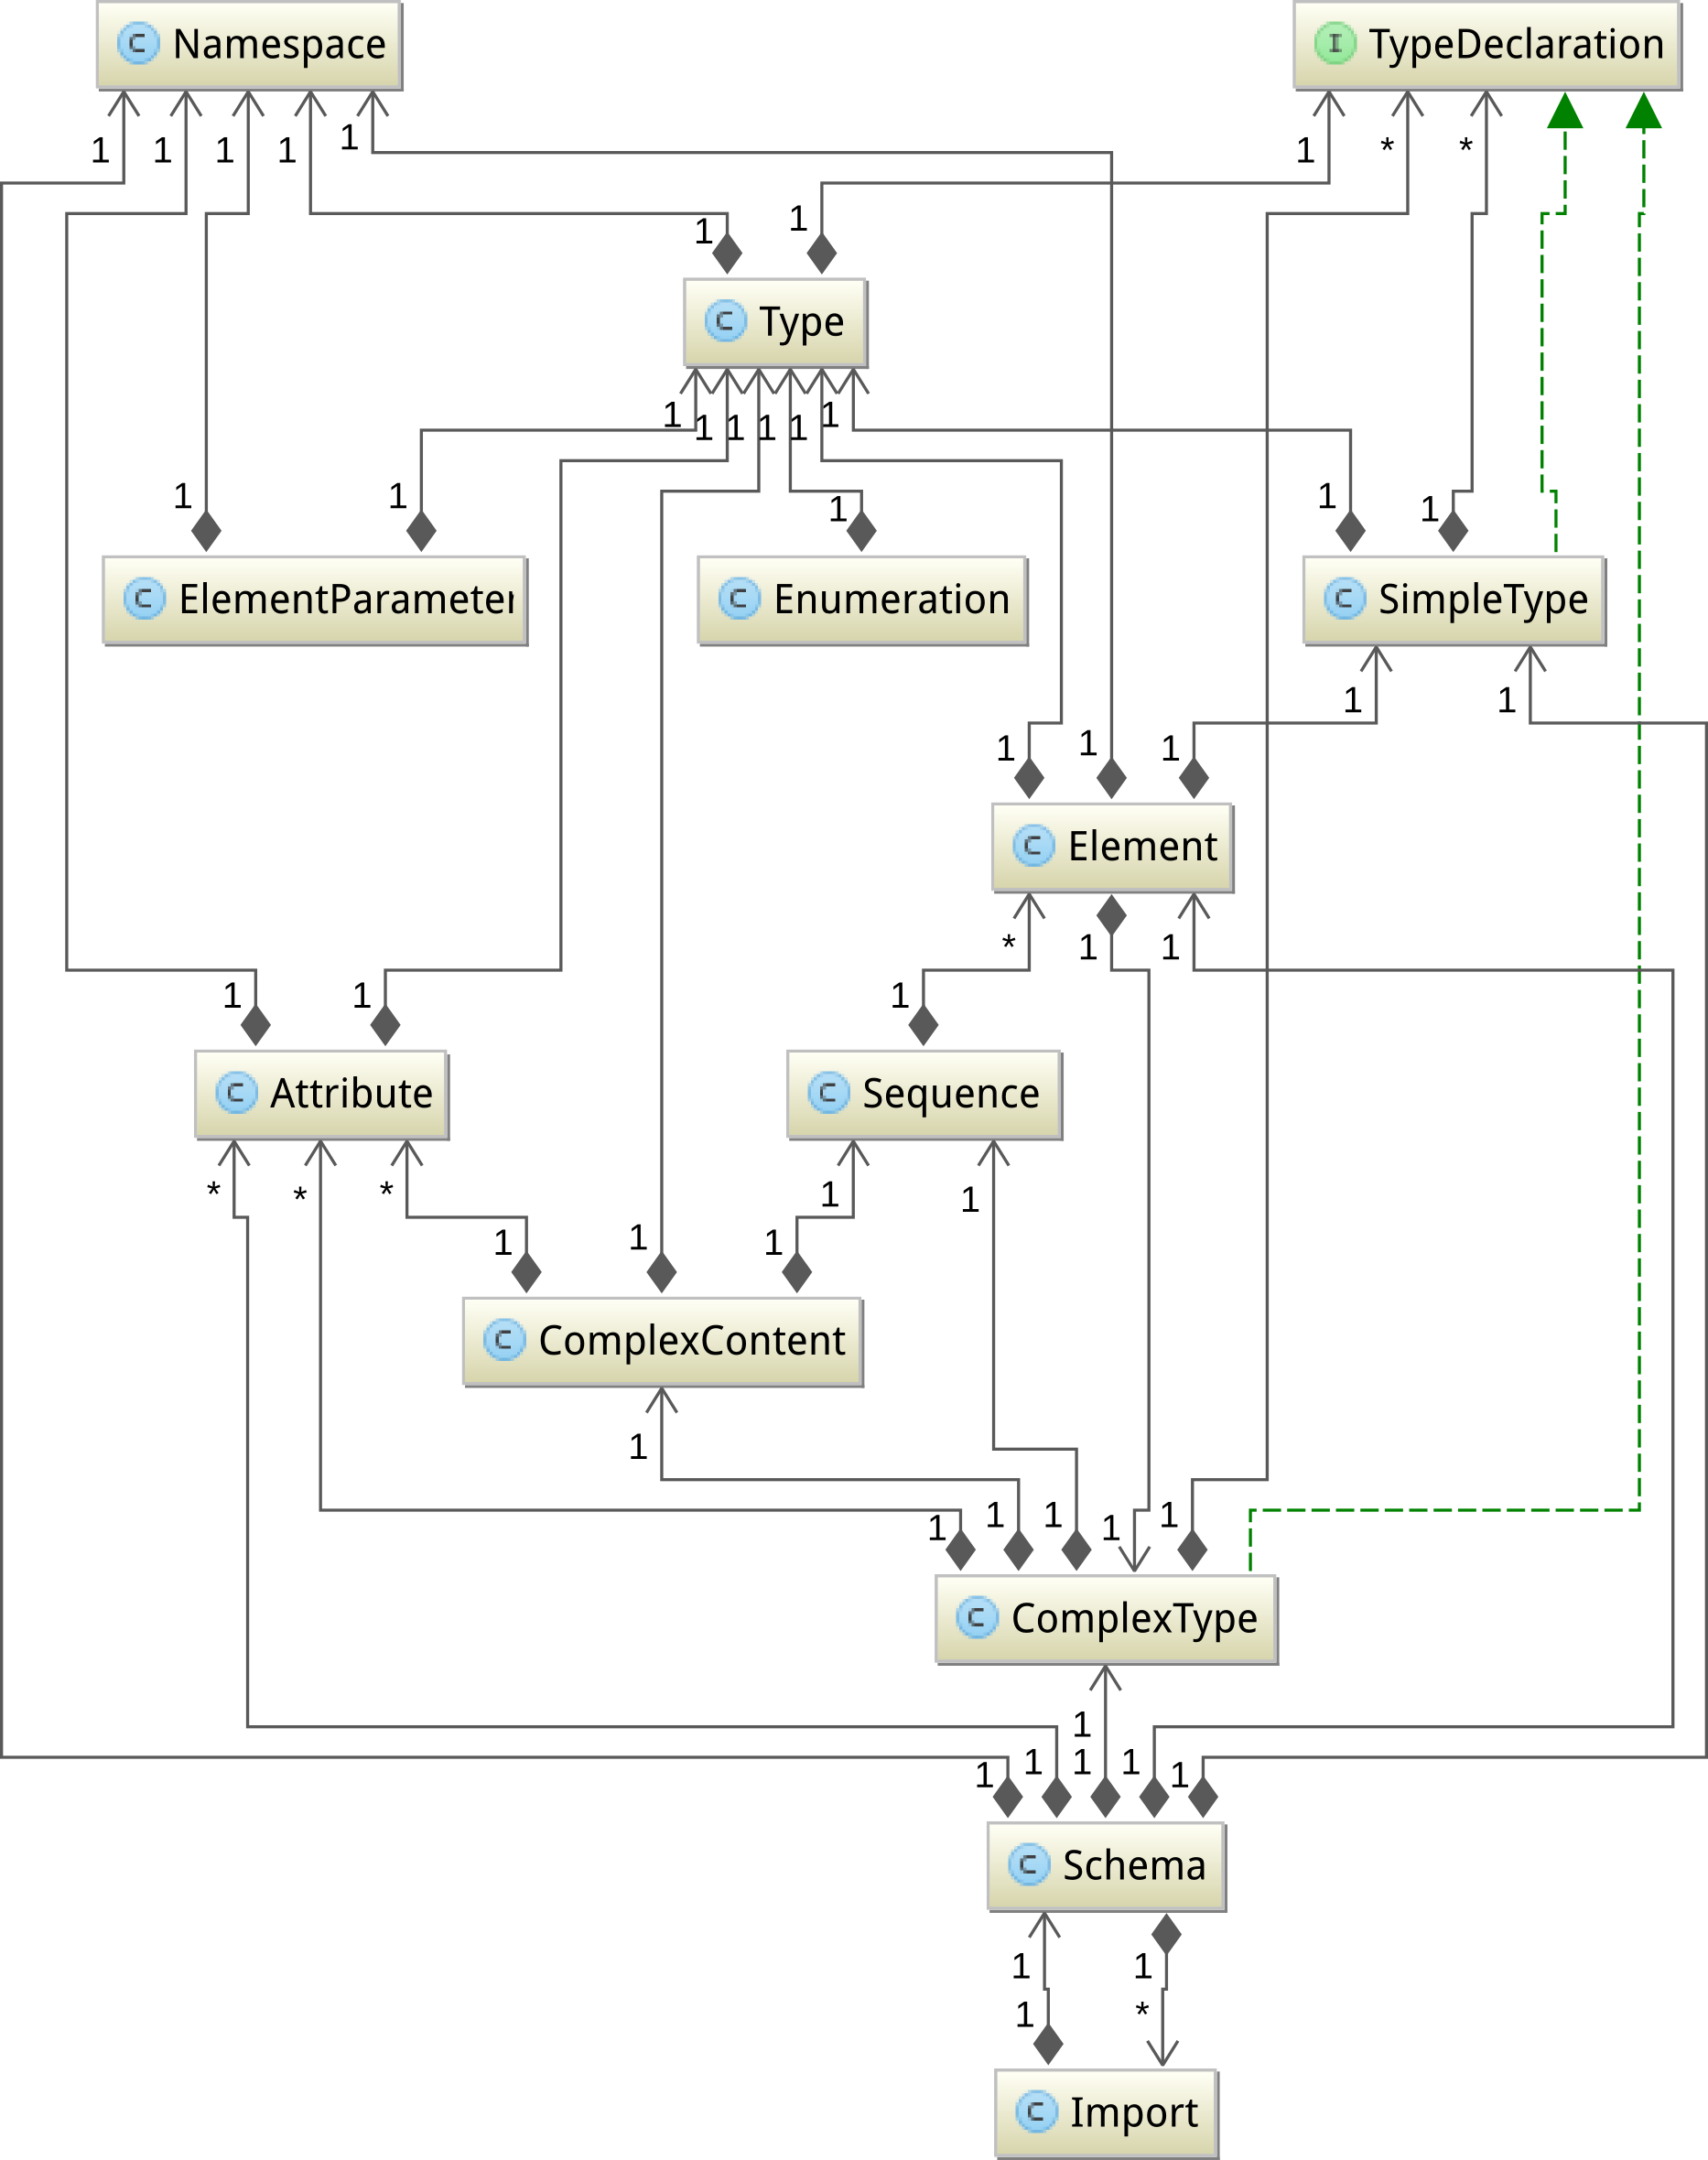
\includegraphics[width=0.6\textwidth]{resources/typemodel}
    \caption{\textsc{Uml} Klassendiagramm des Schemadatenmodells}
    \label{fig:schema_model}
\end{figure}

Wurzel des Schemadatenmodells ist die Klasse \textbf{Schema}. Ein Schema kann Objekte vom Typ \emph{Complex-} und \emph{SimpleType} sowie \emph{Attribute} und \emph{Element} enthalten.

\gls{XSD}-Dateien erlauben das Importieren anderer Schemadefinitionen, die Klasse \textbf{Import} ermöglicht dies im Schemamodell. Sie besitzt ein Objekt des zu importierenden Schemas sowie eine \gls{URI} auf die zugehörige \gls{XSD}-Datei.

Primitive Schematypen werden durch die Klasse \emph{SimpleType} abgebildet. Objekte dieser Klasse enthalten eine Kennzeichnung der Art des SimpleType (Enumerator, Liste, einfacher Wert) und bei Enumeratoren zusätzlich die einzelnen Enumeratorwerte sowie die Angabe des Basisdatentyps.

Die \textbf{ComplexType}-Klasse repräsentiert die gleichnamigen strukturierten Typen aus der Schemabeschreibung. 
Ein ComplexType kann Attribute, Elemente, Elementsequenzen und strukturierten Inhalt (\emph{ComplexContent}) enthalten.

\textbf{ComplexContent} kann die gleichen Objekte wie \emph{ComplexType} enthalten, sowie einen Basistyp der erweitert oder eingeschränkt wird (\enquote{derivation by extension/restriction}).

Attribute werden durch die gleichnamige Klasse \textbf{Attribute} gekapselt, sie besitzen einen Attributnamen sowie eine Definition ihres Typs.

Elementsequenzen werden durch die \textbf{Sequence}-Klasse repräsentiert. Sie enthält einen Reihenfolgeindikator und die Elemente der Sequenz.

Objekte der Klasse \textbf{Element} besitzen einen Bezeichner sowie einen Complex- oder SimpleType und optional eine Angabe der Auftrittshäufigkeit. Die Klasse \emph{ElementParameter} dient nur zur Kapselung der Daten, welche an den Konstruktor der Elementklasse gegeben werden.

Durch die Klasse \textbf{Namespace} werden der Namensraumbezeichner und der konkrete Namensraum eines Typs aus dem Schema gekapselt. 

\begin{figure}[ht]
    \centering
    \begin{minipage}[b]{0.6\linewidth}
        \begin{lstlisting}[
            language=XML,
            label=lst:xsdExamplePoint,                
            numbers=none,
            xleftmargin=0mm,
            framexleftmargin=2mm,
        ]
<xs:element 
    xmlns:tns="http://api.spreadshirt.net" 
    type="tns:point" name="point"/>

<xs:complexType name="point">
    <xs:sequence>
        <xs:element 
            type="xs:double" name="x"/>
        <xs:element 
            type="xs:double" name="y"/>
    </xs:sequence>
    <xs:attribute 
        xmlns:tns="http://api.spreadshirt.net" 
        type="tns:unit" name="unit"/>
</xs:complexType>
        \end{lstlisting}
    \end{minipage}
    \quad    
    \begin{minipage}[b]{0.35\linewidth}
        \begin{tikzpicture}[every tree node/.style={font=\footnotesize}]
            \Tree
            [
                .Element
                [
                    .ComplexType
                    [ . Attribute ]
                    [ .Sequence 
                        Element
                        [ .Element ]
                    ]
                ]
            ]
        \end{tikzpicture}
        %\label{fig:minipage2}
    \end{minipage}
    \caption{Datentyp Point mit Gegenüberstellung im Schemamodell}
\end{figure}

\subsection{Applikationsmodell}
\label{sec:application_model}

Das Applikationsmodell ist die Gesamtheit des REST- und Schemamodells. Referenzen auf Typenbeschreibungen im REST-Modell werden durch deren Definition im Schemamodell ersetzt. Dieses gemeinsame Modell dient dem Generator als Eingabequelle.

\subsection{Sprachenmodell}
\label{sec:language_model}

% Bild aktualisieren
\begin{sidewaysfigure}[tb]
    \centering
    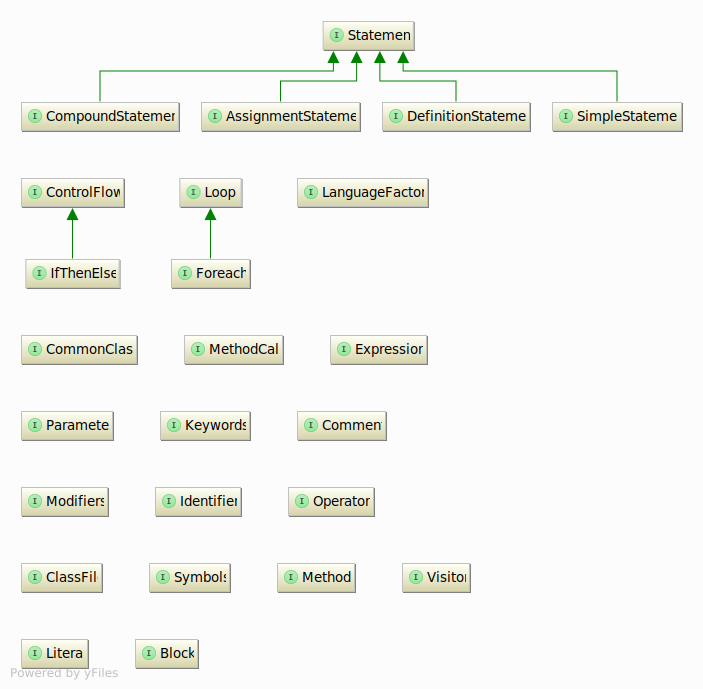
\includegraphics[width=\textwidth]{resources/languagemodel_common}
    \caption{UML Klassendiagramm des Zielsprachenmodells}
    \label{fig:language_model}
\end{sidewaysfigure}

Die Aufgabe des Generators ist die Transformierung des Applikationsmodells in das Modell der Zielsprache. 

Um die gewünschte Austauschbarkeit der Zielsprache zu gewährleisten wurde ein abstraktes Sprachenmodell entworfen welches die Konstrukte einer dateibasierten Objektorientierten Programmiersprache (siehe \cref{sec:oo_languages}) abbildet. 
%Anforderungen erstellen und referenzieren.
Die gewünschte Zielsprache muss dabei die Klassen und Methoden des Modells implementieren sowie eine \emph{Language Factory} (siehe \cref{sec:language_factory}) bereitstellen um vom Generator genutzt werden zu können.

Syntax ist kein Bestandteil des Modells sondern wird von einem \emph{LanguageVisitor} (siehe \cref{sec:language_visitor}) implementiert, das Sprachenmodell enthält nur die nötigen \emph{accept}-Methoden für den Visitor.

Basis des Modells ist die Klasse \textbf{ClassFile}, sie abstrahiert eine Klassendatei mit den Eigenschaften:
\begin{compactitem}
    \item Dateiname
    \item Namensraum
    \item Liste von Abhängigkeiten (\emph{Dependency}-Klasse)
    \item Klassendefinition
\end{compactitem}

Die Liste von Abhängigkeiten der zu generierenden Klassen muss vorher aus dem Eingabemodell ermittelt werden, dies geschieht durch Analyse der in den Elementdefinitionen des Schemamodells enthaltenen Typen. 

% Modifier sind Schlüsselwörter einer Sprache die deren Verhalten ändern.

\textbf{Keywords} und \textbf{Symbols} dienen zur Kapselung der Schlüsselwörter und Symbole einer Sprache. Keywords enthält Methoden zur Abfrage typischer Schlüsselworte wie \emph{class}, \emph{import}, \emph{new} oder \emph{this}. Sprachspezifische Symbole wie \emph{Verkettungs}- und \emph{Scope}-Operatoren oder Präfixe für Variablennamen können über Methoden der Klasse Symbols vom Generator abgefragt werden.

\subsection{Language Visitor}
\label{sec:language_visitor}

Kapitel gehört eher zu Generator

% Sprachschnittstelle!
\subsection{Language Factory}
\label{sec:language_factory}

Um eine Zielsprachenunabhänhigkeit zu erreichen, wird dem Generator bei der Erzeugung eine \enquote{Language Factory} übergeben. Der Generator erzeugt Sprachelemente nur über diese Factory. Ein Aufruf einer Factorymethode gibt ein Element der vom Typ der Sprache zurück, der Generator kennt aber nur den Interface-Typ. Für ihn ist die konkrete Implementierung somit transparent.
